% ============================================================
%  chapter2_slides.tex
%  Chapter 2: Background to Bayesian Machine Learning
%             in Quantitative Finance
%  Bayesian Machine Learning in Quantitative Finance:
%  Theory and Practical Applications
%  Mongwe, Mbuvha & Marwala --- Springer, 2025
% ============================================================
\documentclass[aspectratio=169,10pt]{beamer}

\usetheme{Madrid}
\usecolortheme{seahorse}
\usefonttheme{professionalfonts}

% -- packages ------------------------------------------------------------------
\usepackage{amsmath,amssymb,bm}
\usepackage{graphicx}
\usepackage{booktabs}
\usepackage{listings}
\usepackage{xcolor}
\usepackage{tikz}
\usetikzlibrary{shapes,arrows,positioning,calc}
\usepackage{mathtools}
\usepackage{array}
\usepackage{multirow}

\graphicspath{{figures/}}

% -- listings style --------------------------------------------------------
\lstdefinestyle{pythonstyle}{
  language=Python,
  basicstyle=\ttfamily\scriptsize,
  keywordstyle=\color{blue}\bfseries,
  stringstyle=\color{orange},
  commentstyle=\color{green!50!black}\itshape,
  numberstyle=\tiny\color{gray},
  numbers=left,
  stepnumber=1,
  numbersep=5pt,
  frame=single,
  backgroundcolor=\color{gray!7},
  breaklines=true,
  showstringspaces=false,
  tabsize=2,
  captionpos=b,
}
\lstset{style=pythonstyle}

% -- beamer setup -----------------------------------------------------------
\setbeamertemplate{footline}[frame number]
\setbeamertemplate{navigation symbols}{}
\setbeamersize{text margin left=0.5cm, text margin right=0.5cm}

% -- title -------------------------------------------------------------------
\title[Bayesian ML in QF -- Ch.2]{Bayesian Machine Learning in Quantitative Finance}
\subtitle{Chapter 2: Background}
\author{Based on Mongwe, Mbuvha \& Marwala}
\institute{Springer, 2025}
\date{}

% =============================================================================
\begin{document}
% =============================================================================

\begin{frame}
  \titlepage
\end{frame}

\begin{frame}{Chapter Outline}
  \tableofcontents
\end{frame}

% =============================================================================
\section{2.1 Introduction}
% =============================================================================

\begin{frame}[allowframebreaks]{Two Ways to Do Statistics: Frequentist vs.\ Bayesian}
  \textbf{Intuition first.} Suppose you want to know how likely a coin is to
  land heads. There are two fundamentally different philosophies about what
  ``probability'' even means here, and they lead to two different styles of
  inference.

  \begin{block}{Frequentist inference}
    Probability is a \emph{long-run frequency}: ``the probability of heads is
    $0.6$'' means ``if I flipped this coin infinitely many times, $60\%$ of
    flips would be heads.'' Model parameters are treated as \emph{fixed but
    unknown constants}. We estimate them with a single ``best guess'' (a
    point estimate) computed from the observed data.
  \end{block}

  \begin{block}{Bayesian inference}
    Probability also describes a \emph{degree of belief}. Model parameters
    are treated as \emph{random variables} with their own distribution. We
    start with a prior belief, update it with observed data via Bayes'
    theorem, and end up with a full \emph{posterior distribution} over the
    parameter -- not just one number.
  \end{block}

  \framebreak

  \textbf{A little history.} Bayesian inference is actually \emph{older}
  than the frequentist paradigm, but it was neglected for a long time. The
  primary reason: Bayesian statistics could only be applied in a limited
  number of situations where a conjugate prior was known in closed form; when
  no closed-form posterior was available, the method stalled.

  The resurgence of Bayesian statistics in recent decades is attributed to:
  \begin{itemize}
    \item the rapid growth of \textbf{computational power} and \textbf{data
      volume}, and
    \item the development of novel mathematical algorithms -- most notably
      \textbf{Markov Chain Monte Carlo (MCMC)} techniques, developed in the
      1950s, including the Hastings (1970) algorithm.
  \end{itemize}
  MCMC made it possible to build random sampling algorithms for a probability
  distribution and compute Bayesian hierarchical models even when no
  closed-form posterior exists. A few years later, statisticians began
  routinely using MCMC, marking the start of the contemporary Bayesian
  statistics era.

  \framebreak

  \textbf{Criticisms on both sides.} Neither paradigm is free of
  controversy:
  \begin{itemize}
    \item Frequentist hypothesis testing is frequently criticized for its use
      of $p$-values, which are partially based on data that were
      \emph{never actually observed} (hypothetical repeated sampling).
    \item Bayesian methods do not use null/alternative hypotheses at all, so
      that particular criticism does not apply to them. Instead, the main
      criticism of Bayesian methods is the \textbf{subjectivity of the
      chosen prior distribution}: there is no single, well-defined,
      recommended way to pick a prior, so different studies may choose
      different priors for the same experiment and reach different
      conclusions.
    \item In defence of Bayesian methods: as long as the prior is
      appropriately specified, validity is preserved regardless of the
      experimental design, and Bayesian techniques merely ascertain an
      event's likelihood. Trying several different priors also lets us
      measure how \emph{sensitive} our conclusions are to prior
      assumptions.
  \end{itemize}

  \framebreak

  \textbf{Why this book uses the Bayesian paradigm.} The Bayesian framework
  lets us naturally answer questions that matter a great deal in
  quantitative finance:
  \begin{itemize}
    \item How can we explain the prediction or output of a model?
    \item What is the distribution of the model's parameters (i.e.\ how
      \emph{uncertain} are we about them)?
    \item How do we select between different models in a statistically
      principled manner?
    \item Which inputs are most relevant to the task at hand?
  \end{itemize}
  The Bayesian framework is founded on \textbf{Bayes' theorem}, which lets us
  update prior beliefs through new observations, encapsulated through the
  assumed underlying model. The rest of this chapter builds up the
  vocabulary needed for every later chapter in this book.
\end{frame}

% -----------------------------------------------------------------------------
\begin{frame}[allowframebreaks]{Notation You'll Need: A Glossary for the Rest of This Book}
  This chapter introduces several terms that will be used, without
  re-explanation, in every subsequent chapter. Read this glossary carefully.

  \begin{block}{Bayesian Machine Learning (BML)}
    Ordinary (``frequentist'') machine learning fits a model and returns
    \emph{one best-fit answer} for each parameter and each prediction.
    \textbf{Bayesian machine learning blends computational models with
    Bayesian inference}: it fits the model \emph{and} returns a full
    \emph{distribution} describing how uncertain we are about every
    parameter and every prediction. Analogy: instead of a weather forecaster
    saying ``it will be $23^\circ$C tomorrow'' (a point estimate), a Bayesian
    forecaster says ``there's a range of likely temperatures, centred around
    $23^\circ$C, and here is exactly how spread out that range is.''
  \end{block}

  \begin{block}{Prior, Likelihood, Posterior (recap)}
    \begin{itemize}
      \item \textbf{Prior} $\mathbb{P}(\mathbf{w})$: what we believe about
        the parameters $\mathbf{w}$ \emph{before} seeing any data.
      \item \textbf{Likelihood} $\mathbb{P}(D\mid \mathbf{w})$: how probable
        the observed data $D$ is, for a given setting of $\mathbf{w}$.
      \item \textbf{Posterior} $\mathbb{P}(\mathbf{w}\mid D)$: what we
        believe about $\mathbf{w}$ \emph{after} seeing the data $D$ --
        obtained by combining the prior and the likelihood via Bayes'
        theorem.
    \end{itemize}
    Analogy: a detective (prior suspicion) updates their beliefs about
    ``who did it'' as new evidence (likelihood of the evidence given each
    suspect) comes in, arriving at a final, evidence-weighted verdict
    (posterior).
  \end{block}

  \framebreak

  \begin{block}{Markov Chain Monte Carlo (MCMC) -- high-level idea}
    Very often, the posterior distribution cannot be written down in closed
    form. \textbf{MCMC is a way to draw samples from a complicated posterior
    distribution you can't write down in closed form, by running a
    cleverly designed random walk} whose long-run behaviour matches that
    posterior. Instead of computing the posterior analytically, we generate
    a long sequence of parameter values (a ``chain'') such that, after
    enough steps, the values visited are distributed \emph{as if} drawn
    directly from the true posterior. We will make this precise (the
    Metropolis-Hastings algorithm) later in this chapter.
  \end{block}

  \begin{block}{Gaussian Process (GP) -- previewed here, used in later chapters}
    A Gaussian process is a \textbf{``distribution over functions''}: a
    flexible, non-parametric Bayesian model. Instead of assuming the
    relationship between inputs and outputs has a fixed parametric form
    (like a straight line), a GP places a prior directly over the space of
    possible functions, and Bayes' theorem updates this prior into a
    posterior distribution over functions that are consistent with the
    observed data points. Analogy: rather than fitting one curve, imagine an
    infinite bundle of candidate curves, each with a plausibility weight; the
    GP keeps track of that whole weighted bundle, and shrinks the bundle
    around the data points that have been observed.
  \end{block}

  \framebreak

  \begin{block}{Normalizing Flow -- previewed here, used in later chapters}
    A normalizing flow is \textbf{a way to build complex, flexible
    probability distributions by transforming a simple one, like a
    Gaussian, through a sequence of invertible functions}. Because each
    transformation is invertible (and its Jacobian determinant is easy to
    compute), we can start with an easy distribution (e.g.\ a standard
    Gaussian), push samples through a chain of learned transformations, and
    end up with samples from a much richer, more realistic distribution --
    while still being able to evaluate exact densities. Analogy: think of
    modelling clay (the simple Gaussian) that gets pushed, stretched, and
    twisted by a sequence of reshaping tools (the invertible transforms)
    into an intricate final sculpture (the complex target distribution).
  \end{block}

  \begin{block}{Bayesian Neural Network (BNN) -- previewed here, used in later chapters}
    An ordinary neural network learns one fixed number for every weight. A
    \textbf{Bayesian neural network is a neural network whose weights are
    themselves treated as uncertain, with a distribution over them, not
    fixed numbers}. Training a BNN means inferring a posterior distribution
    over all of the network's weights given the data, instead of finding a
    single ``best'' weight vector. Predictions are then made by averaging
    over many plausible networks (one per weight sample), which naturally
    produces a measure of predictive uncertainty alongside the prediction
    itself.
  \end{block}
\end{frame}

% -----------------------------------------------------------------------------
\begin{frame}[fragile]{Python: Frequentist Point Estimate vs.\ Bayesian Posterior}
  \textbf{Goal:} on 5 coin flips (H, T, H, H, T), contrast a frequentist
  point estimate with a full Bayesian posterior.
  \begin{lstlisting}
import numpy as np
from scipy.stats import beta

data = [1, 0, 1, 1, 0]        # H,T,H,H,T encoded as 1/0
n = len(data)
n_heads = sum(data)                 # 3
n_tails = n - n_heads                # 2

# --- Frequentist: Maximum Likelihood Estimate (MLE) ---
theta_mle = n_heads / n
print(f"Frequentist point estimate: theta_MLE = {theta_mle:.4f}")

# --- Bayesian: Beta(1,1) uniform prior -> Beta posterior ---
a_prior, b_prior = 1.0, 1.0
a_post, b_post = a_prior + n_heads, b_prior + n_tails   # Beta(4,3)
post_mean = a_post / (a_post + b_post)
ci_low, ci_high = beta.ppf([0.025, 0.975], a_post, b_post)

print(f"Bayesian posterior: Beta({a_post:.0f},{b_post:.0f})")
print(f"  mean = {post_mean:.4f}, 95% CI = [{ci_low:.4f}, {ci_high:.4f}]")
  \end{lstlisting}
  \textbf{Output:} {\ttfamily theta\_MLE = 0.6000}; Bayesian posterior
  {\ttfamily Beta(4,3)}, mean $=0.5714$, 95\% CI $=[0.2228,\,0.8819]$. Same
  data, one number vs.\ a whole distribution with a quantified uncertainty.
\end{frame}

% -----------------------------------------------------------------------------
\begin{frame}[allowframebreaks]{2.1.1 Bayesian Machine Learning}
  \textbf{Definition.} To produce predictions \emph{and} their associated
  uncertainties, Bayesian machine learning blends computational models with
  the ideas of Bayesian inference. Its foundation is the Bayesian framework,
  which enables modelling uncertainty and updating beliefs in light of
  observed data and past knowledge. Bayesian machine learning combines
  probability distributions over model parameters \emph{and} predictions,
  offering a more thorough account of uncertainty than classic machine
  learning techniques, which only produce point estimates.

  \begin{block}{Benefits}
    \begin{itemize}
      \item Flexible modelling.
      \item The capacity to incorporate prior information.
      \item Systematic, principled treatment of uncertainty.
    \end{itemize}
  \end{block}

  \framebreak

  \begin{block}{Difficulties}
    \begin{itemize}
      \item Scalability to large datasets and high-dimensional models.
      \item Computing complexity -- Bayesian posteriors are often expensive
        to obtain.
    \end{itemize}
  \end{block}

  \textbf{Where the field is headed.} Future research in Bayesian machine
  learning aims to:
  \begin{itemize}
    \item develop scalable algorithms,
    \item increase computational efficiency,
    \item bridge the gap between Bayesian approaches and deep learning, and
    \item address interpretability difficulties.
  \end{itemize}

  In general, Bayesian machine learning offers a practical paradigm for
  describing uncertainty and producing well-informed predictions in machine
  learning tasks. The next table summarizes how it compares to the classic
  (frequentist) paradigm across five practical dimensions.
\end{frame}

% -----------------------------------------------------------------------------
\begin{frame}{Table 2.1: Frequentist vs.\ Bayesian Machine Learning}
  \small
  \begin{tabular}{p{2.4cm}p{4.6cm}p{4.6cm}}
    \toprule
    \textbf{Metric} & \textbf{Frequentist} & \textbf{Bayesian} \\
    \midrule
    Uncertainty Quantification &
      No natural notion of uncertainty -- predictions are point estimates &
      Captures uncertainty in parameters and predictions through
      probability distributions \\[2pt]
    Prior Beliefs &
      No notion of a prior; cannot naturally incorporate prior beliefs &
      A prior distribution captures beliefs about parameters, updated via
      Bayes' theorem \\[2pt]
    Regularization \& Over-fitting &
      No natural regularization; the user must select a penalty by hand &
      Prior distributions over parameters naturally regularize, reducing
      over-fitting \\[2pt]
    Model Selection &
      Usually via $K$-fold cross-validation or leave-one-out; no agreed
      state-of-the-art metric &
      The Bayesian evidence (the posterior's normalizing constant) gives a
      principled way to compare models \\[2pt]
    Scalability &
      Scales more easily to huge dimensions and datasets &
      Often computationally demanding; can be difficult to scale to large
      datasets \\
    \bottomrule
  \end{tabular}
\end{frame}

% =============================================================================
\section{2.1.2 Bayesian ML Models}
% =============================================================================

\begin{frame}[allowframebreaks]{2.1.2 Bayesian Machine Learning Models: An Overview}
  Bayesian machine learning contains an assortment of methodologies that
  apply Bayesian principles to draw inferences and make predictions. This
  book uses the following model classes.

  \begin{block}{Bayesian Logistic Regression}
    Adds prior distributions over the parameters of classical logistic
    regression. In light of the observed data, it offers a
    \emph{posterior distribution} across the parameters and quantifies
    uncertainty in the parameter estimates (rather than a single fitted
    coefficient vector).
  \end{block}

  \begin{block}{Bayesian Mixture Models}
    Probabilistic models that assume the data is generated from a
    combination of underlying distributions. They handle uncertainty in the
    model parameters and enable density estimation and clustering by
    imposing priors on the mixture proportions and on the parameters of each
    component distribution.
  \end{block}

  \framebreak

  \begin{block}{Gaussian Processes (GPs)}
    Non-parametric models that are flexible and describe a
    \emph{prior distribution over functions} (see the glossary earlier in
    this chapter). GPs can identify intricate patterns in the data and
    offer estimates of prediction uncertainty. Common uses: regression,
    classification, and time series analysis.
  \end{block}

  \begin{block}{Bayesian Neural Networks (BNNs)}
    Add prior distributions over the network weights, expanding on the
    architecture of classical (frequentist) neural networks. BNNs can
    estimate posterior distributions over the weights using methods like
    variational inference or MCMC sampling, allowing for
    \textbf{Bayesian model averaging} and uncertainty quantification.
  \end{block}

  \framebreak

  \begin{block}{Bayesian Formulation of Economic Models}
    Sometimes a traditional (frequentist) model from quantitative finance --
    for example, the Heston stochastic volatility model -- is instead framed
    within the Bayesian framework, so that its parameters get a full
    posterior distribution rather than a single calibrated value. These
    models are explored in detail in the relevant application chapters of
    this book.
  \end{block}

  \textbf{Looking ahead.} Two further tools appear repeatedly in later
  chapters of this book even though they are not part of this introductory
  list: \textbf{normalizing flows} (for building flexible, exact-density
  distributions, used e.g.\ for option-price and audit-outcome modelling)
  and, more generally, deep \textbf{Bayesian neural networks} for
  claims/insurance-type problems. Their plain-English definitions are in
  the glossary earlier in this chapter -- the relevant chapters develop the
  full technical machinery.
\end{frame}

% -----------------------------------------------------------------------------
\begin{frame}[fragile]{Python: A Gaussian Process is a ``Distribution over Functions''}
  \textbf{Goal:} draw one random function from a GP prior with a
  radial-basis-function (RBF) kernel, to make the ``distribution over
  functions'' idea concrete.
  \begin{lstlisting}
import numpy as np

def rbf_kernel(x1, x2, length_scale=1.0, variance=1.0):
    sq_dist = (x1[:, None] - x2[None, :]) ** 2
    return variance * np.exp(-0.5 * sq_dist / length_scale**2)

x = np.linspace(-3, 3, 50)
K = rbf_kernel(x, x) + 1e-6 * np.eye(len(x))   # jitter for stability
L = np.linalg.cholesky(K)                       # K = L L^T

rng = np.random.default_rng(0)
z = rng.standard_normal(len(x))       # standard normal "noise"
f_sample = L @ z                      # one random FUNCTION, f(x) for all x

print("A single draw from GP(0, K) at 5 grid points:")
print(np.round(f_sample[::10], 3))
  \end{lstlisting}
  Every re-run of \texttt{rng.standard\_normal} produces an \emph{entire new
  curve} $f(x)$ consistent with the kernel's smoothness assumptions --
  literally sampling a function, not a number.
\end{frame}

% =============================================================================
\section{2.1.3 Training Bayesian ML Models}
% =============================================================================

\begin{frame}[allowframebreaks]{2.1.3 Training Bayesian Machine Learning Models}
  The Bayesian framework, and hence Bayesian machine learning, is founded on
  Bayes' theorem, which states that for a given model $M$ with parameters
  $\mathbf{w}$ and data $D$:

  \begin{block}{Bayes' Theorem for Model Parameters}
    \[
      \underbrace{\mathbb{P}(\mathbf{w}\mid D, M)}_{\text{posterior}}
      = \frac{\overbrace{\mathbb{P}(D\mid \mathbf{w}, M)}^{\text{likelihood}}\
              \overbrace{\mathbb{P}(\mathbf{w}\mid M)}^{\text{prior}}}
             {\underbrace{\mathbb{P}(D\mid M)}_{\text{evidence}}}
      \tag{2.1}
    \]
    \begin{itemize}
      \item $\mathbb{P}(\mathbf{w}\mid D,M)$ -- the \textbf{posterior}: what
        we believe about the parameters after seeing the data.
      \item $\mathbb{P}(D\mid \mathbf{w},M)$ -- the \textbf{likelihood}: how
        probable the data $D$ is, for a given $\mathbf{w}$.
      \item $\mathbb{P}(\mathbf{w}\mid M)$ -- the \textbf{prior}: what we
        believe about $\mathbf{w}$ before seeing $D$.
      \item $\mathbb{P}(D\mid M)$ -- the \textbf{Bayesian evidence} (or
        marginal likelihood) for model $M$; a normalizing constant that can
        also be used for model selection.
    \end{itemize}
  \end{block}

  A Bayesian model is fully specified once the prior $\mathbb{P}(\mathbf{w}\mid M)$
  and the likelihood $\mathbb{P}(D\mid \mathbf{w},M)$ have been chosen. The
  prior is typically a Gaussian distribution (sometimes with a different
  standard deviation per parameter). The likelihood is typically the
  Bayesian analogue of whatever loss function would have been used in
  frequentist inference -- e.g.\ for a regression problem, the likelihood
  corresponds to the least-squares error.

  \framebreak

  \textbf{Why we need numerical methods.} The aim of training a Bayesian
  machine learning model is to infer the posterior
  $\mathbb{P}(\mathbf{w}\mid D,M)$. This posterior is typically \emph{not}
  available in closed form, because the Bayesian evidence
  $\mathbb{P}(D\mid M)$ is itself usually intractable (it requires
  integrating the numerator of Eq.~(2.1) over all possible $\mathbf{w}$).
  Numerical techniques are therefore required. The two common families of
  approaches, both of which amount to determining the posterior distribution
  within the Bayesian framework, are:
  \begin{itemize}
    \item \textbf{Variational Inference (VI)} -- turns the sampling problem
      into an optimization problem.
    \item \textbf{Markov Chain Monte Carlo (MCMC)} -- draws samples directly
      via a guided random walk.
  \end{itemize}
  MCMC algorithms are generally preferable in that they converge to the
  \emph{correct} target distribution if the sample size is sufficiently
  large, whereas MCMC's main disadvantage is slow execution compared to
  variational methods. Typically, neither family simultaneously estimates
  the Bayesian evidence \emph{and} the posterior during inference -- the
  evidence is usually only computed afterwards, as a post-processing step
  (although some methods, such as nested sampling, aim to estimate the
  evidence directly and produce the posterior as a by-product).

  \textit{A remark on scope:} this chapter (and this book) focuses on VI and
  MCMC as the two training paradigms. A third approximate technique you may
  encounter elsewhere in the wider Bayesian machine learning literature is
  the \textbf{Laplace approximation}, which fits a Gaussian centred at the
  posterior mode using the local curvature there; it is fast but is not
  developed further in this chapter.
\end{frame}

% -----------------------------------------------------------------------------
\begin{frame}[allowframebreaks]{Worked Example: MLE vs.\ Bayesian Posterior, by Hand}
  \textbf{Setup.} 5 coin flips: H, T, H, H, T $\;\Rightarrow\;$ 3 heads, 2
  tails ($n=5$). Model: each flip is Bernoulli$(\theta)$ with
  $\theta = \mathbb{P}(\text{heads})$.

  \begin{block}{Step 1 -- Frequentist point estimate (MLE)}
    The likelihood of the data is
    $\mathbb{P}(D\mid\theta) = \theta^{3}(1-\theta)^{2}$.
    Maximizing over $\theta$ (set derivative of the log-likelihood to zero)
    gives
    \[
      \hat\theta_{MLE} = \frac{n_{\text{heads}}}{n} = \frac{3}{5} = 0.6 .
    \]
    This single number is the frequentist's entire answer -- no uncertainty
    is attached to it.
  \end{block}

  \framebreak

  \begin{block}{Step 2 -- Bayesian posterior (Beta-Bernoulli conjugacy)}
    Choose a uniform prior $\theta \sim \text{Beta}(\alpha_0{=}1,\beta_0{=}1)$
    (i.e.\ we believe every value of $\theta \in [0,1]$ is equally likely
    beforehand). The Beta distribution is \emph{conjugate} to the Bernoulli
    likelihood, so the posterior is again Beta, with parameters updated by
    simply adding the observed counts:
    \[
      \alpha_{\text{post}} = \alpha_0 + n_{\text{heads}} = 1 + 3 = 4, \qquad
      \beta_{\text{post}} = \beta_0 + n_{\text{tails}} = 1 + 2 = 3 .
    \]
    So $\theta \mid D \sim \text{Beta}(4,3)$: a whole distribution, not a
    single number.
  \end{block}

  \framebreak

  \begin{block}{Step 3 -- Reading off numbers from the posterior}
    \[
      \mathbb{E}[\theta\mid D] = \frac{\alpha_{\text{post}}}{\alpha_{\text{post}}+\beta_{\text{post}}}
      = \frac{4}{7} \approx 0.5714, \qquad
      \text{mode} = \frac{\alpha_{\text{post}}-1}{\alpha_{\text{post}}+\beta_{\text{post}}-2}
      = \frac{3}{5} = 0.6 .
    \]
    \[
      \text{Var}(\theta\mid D) = \frac{\alpha_{\text{post}}\,\beta_{\text{post}}}
        {(\alpha_{\text{post}}+\beta_{\text{post}})^2(\alpha_{\text{post}}+\beta_{\text{post}}+1)}
      = \frac{12}{392} \approx 0.0306, \quad \text{std} \approx 0.175 .
    \]
    A $95\%$ credible interval (computed from the Beta quantiles) is
    approximately $[0.223,\ 0.882]$.
  \end{block}

  \textbf{Contrast.} The posterior \emph{mode} ($0.6$) exactly matches the
  frequentist MLE -- this always happens with a uniform (flat) prior. But
  the Bayesian answer additionally tells us the posterior \emph{mean}
  ($0.5714$) and gives a full quantification of how uncertain we should be
  (std $\approx 0.175$, a wide $95\%$ credible interval) -- information the
  frequentist point estimate simply does not provide.
\end{frame}

% -----------------------------------------------------------------------------
\begin{frame}{Figure: Frequentist Point Estimate vs.\ Bayesian Posterior}
  \centering
  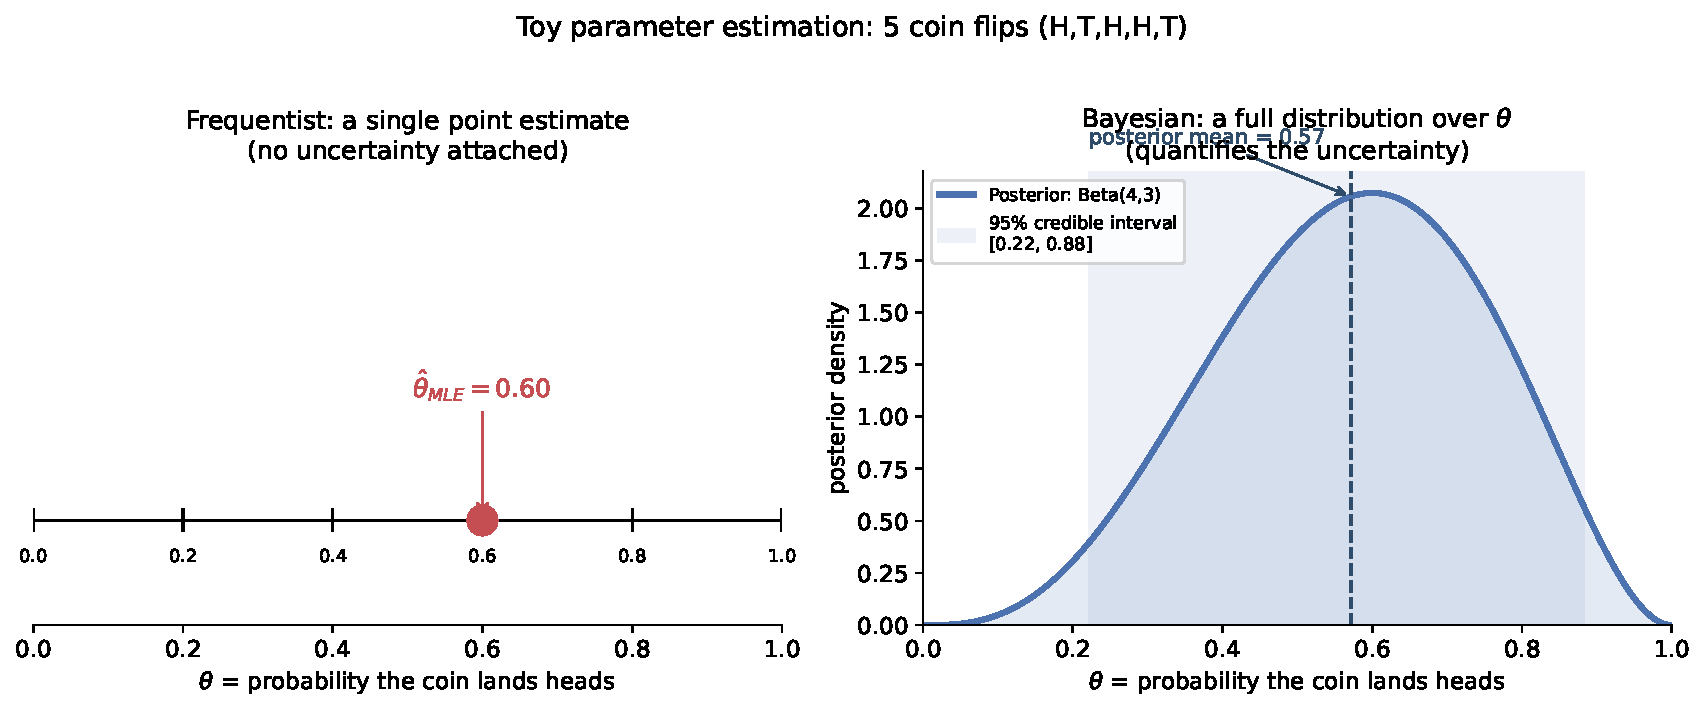
\includegraphics[width=0.95\linewidth]{fig_freq_vs_bayes.pdf}

  \small Left: the frequentist paradigm returns a single point,
  $\hat\theta_{MLE}=0.6$. Right: the Bayesian paradigm returns a full
  posterior density, $\text{Beta}(4,3)$, together with a mean and a $95\%$
  credible interval -- the same 5 coin flips, two very different kinds of
  ``answer.''
\end{frame}

% -----------------------------------------------------------------------------
\begin{frame}[allowframebreaks]{2.1.3.1 Variational Inference: Turning Sampling into Optimization}
  \textbf{Intuition.} When performing Bayesian inference, we want the
  posterior distribution of the model parameters. \textbf{Variational
  inference (VI)} is an approximate inference technique that obtains an
  \emph{approximation} to the true posterior, where the approximation comes
  from a simpler family of distributions (the Gaussian family is a common
  choice, since it is easy to work with mathematically). Through
  approximating with a simpler distribution, the sampling problem is
  transformed into an \emph{optimization} problem: we search for the member
  of the simple family that is closest to the true posterior.

  \textbf{The picture.} We posit a variational family
  $\text{Q}(\mathbf{w},\nu\mid M)$ over the parameters $\mathbf{w}$ for model
  $M$, indexed by variational parameters $\nu$. Starting from initial
  parameters $\nu^0$, an optimization procedure moves $\nu$ toward the
  optimal $\nu^*$ that makes $\text{Q}(\mathbf{w},\nu^*\mid M)$ as close as
  possible (in Kullback-Leibler divergence) to the true posterior
  $\mathbb{P}(\mathbf{w}\mid D,M)$.

  \framebreak

  \begin{block}{Kullback-Leibler (KL) Divergence Objective}
    \[
      KL\big(\text{Q}(\mathbf{w},\nu\mid M)\,\|\,\mathbb{P}(\mathbf{w}\mid D,M)\big)
      = \int \text{Q}(\mathbf{w},\nu\mid M)\,
        \log\!\left[\frac{\text{Q}(\mathbf{w},\nu\mid M)}{\mathbb{P}(\mathbf{w}\mid D,M)}\right] d\mathbf{w}
      \tag{2.2}
    \]
    \begin{itemize}
      \item $\text{Q}(\mathbf{w},\nu\mid M)$ -- the variational
        (approximating) distribution.
      \item $\mathbb{P}(\mathbf{w}\mid D,M)$ -- the true (target) posterior.
      \item $KL(\cdot\|\cdot) \ge 0$, and $KL=0$ only when the two
        distributions are identical.
    \end{itemize}
  \end{block}

  \textbf{The catch:} Eq.~(2.2) still contains the true posterior
  $\mathbb{P}(\mathbf{w}\mid D,M)$, which itself contains the intractable
  Bayesian evidence $\mathbb{P}(D\mid M)$ -- so the KL divergence is not
  directly computable either!

  \framebreak

  \begin{block}{The Evidence Lower Bound (ELBO)}
    Expanding Eq.~(2.2) using $\mathbb{P}(\mathbf{w}\mid D,M) =
    \mathbb{P}(\mathbf{w},D\mid M)/\mathbb{P}(D\mid M)$ and taking
    expectations with respect to $\text{Q}$ gives
    \[
      KL = \underbrace{\mathbb{E}_{\text{Q}}[\log \text{Q}(\mathbf{w},\nu\mid M)]
             - \mathbb{E}_{\text{Q}}[\log \mathbb{P}(\mathbf{w},D\mid M)]}_{-\,\mathbb{L}(D,\nu\mid M)\ (\text{tractable})}
      \;+\; \underbrace{\log \mathbb{P}(D\mid M)}_{\text{intractable}}
      \tag{2.3}
    \]
    where $\mathbb{L}(D,\nu\mid M)$ is the \textbf{evidence lower bound
    (ELBO)}. Since $KL \ge 0$, Eq.~(2.3) shows
    $\log\mathbb{P}(D\mid M) \ge \mathbb{L}(D,\nu\mid M)$ -- the ELBO really
    is a \emph{lower bound} on the log evidence.
  \end{block}

  Because the intractable evidence term does not depend on $\nu$,
  \textbf{maximizing the tractable ELBO} $\mathbb{L}(D,\nu\mid M)$ with
  respect to $\nu$ is \emph{equivalent} to minimizing the KL divergence --
  we have converted an intractable sampling problem into a tractable
  optimization problem. The optimal $\nu^*$ is found by taking the gradient
  of $\mathbb{L}(D,\nu\mid M)$ with respect to $\nu$ and moving in the
  direction of steepest ascent; the exact optimization formulation depends
  on the model $M$ and the chosen family $\text{Q}$.

  \framebreak

  \begin{block}{Variational Inference: Pros and Cons}
    \textbf{Benefits (vs.\ MCMC):}
    \begin{itemize}
      \item Scales more easily to high dimensions.
      \item Enables effective mini-batch optimization for large datasets.
    \end{itemize}
    \textbf{Drawback:} because we restrict ourselves to one \emph{family} of
    parametric distributions, bias is introduced by construction -- in
    general we cannot obtain an exact approximation of the true posterior.
  \end{block}
\end{frame}

% -----------------------------------------------------------------------------
\begin{frame}[allowframebreaks]{2.1.3.2 Markov Chain Monte Carlo: Sampling via a Guided Random Walk}
  Using models with difficult-to-compute posteriors, together with
  approximation procedures to handle them, is the foundation of contemporary
  Bayesian inference. \textbf{MCMC has been the predominant paradigm for
  approximate inference for more than 50 years}: it was first developed in
  the 1940s by scientists including Ulam, Von Neumann, Fermi, and Metropolis.

  \textbf{The MCMC recipe.} We build a Markov chain on the parameters
  $\mathbf{w}$, whose stationary distribution \emph{is} the posterior we
  want. We then take long-run samples from the chain, hoping to gather
  (approximately independent) samples from that stationary distribution.
  MCMC's main drawback is its inability to scale well to high dimensions and
  its comparatively slow execution.

  \framebreak

  \begin{block}{Metropolis-Hastings (MH) Acceptance Rule}
    The seminal, gradient-free Metropolis-Hastings algorithm generates a
    candidate $\mathbf{w}^*$ from a proposal distribution
    $T(\mathbf{w}^*\mid \mathbf{w})$, and accepts or rejects it using the
    ratio of likelihoods:
    \[
      \mathbb{P}(\text{accept } \mathbf{w}^*) =
      \min\left(1,\ \frac{\pi(\mathbf{w}^*)\,T(\mathbf{w}\mid \mathbf{w}^*)}
                          {\pi(\mathbf{w})\,T(\mathbf{w}^*\mid \mathbf{w})}\right)
      \tag{2.4}
    \]
    \begin{itemize}
      \item $\pi(\mathbf{w})$ -- the stationary target density (here, the
        posterior) evaluated at $\mathbf{w}$.
      \item $T(\mathbf{w}^*\mid \mathbf{w})$ -- proposal density for
        moving from the current state $\mathbf{w}$ to the candidate
        $\mathbf{w}^*$.
    \end{itemize}
  \end{block}

  \framebreak

  \begin{block}{Random Walk Metropolis (a common special case)}
    Using a Gaussian proposal centred at the current state,
    $\mathcal{N}(\mathbf{w}, \epsilon\Sigma)$, gives the \textbf{random walk
    Metropolis} algorithm ($\Sigma$ is usually fixed to the identity matrix,
    leaving only the step size $\epsilon$ to tune). Because a Gaussian
    proposal is symmetric, $T(\mathbf{w}\mid\mathbf{w}^*) = T(\mathbf{w}^*\mid\mathbf{w})$,
    so Eq.~(2.4) simplifies to
    \[
      \mathbb{P}(\text{accept } \mathbf{w}^*) = \min\left(1,\ \frac{\pi(\mathbf{w}^*)}{\pi(\mathbf{w})}\right).
      \tag{2.5}
    \]
    Intuition: always move to a candidate that is \emph{more} probable than
    the current state; if it is \emph{less} probable, still move there with
    a probability equal to how much less probable it is (this is what lets
    the chain fully explore the target distribution rather than getting
    stuck on a peak).
  \end{block}

  \framebreak

  \textbf{The drawback of random walk MH.} The proposal density in random
  walk Metropolis-Hastings often induces genuine random-walk behaviour,
  resulting in elevated \textbf{autocorrelations} among the produced
  samples and slow convergence -- large sample sizes are then required
  because high autocorrelations cause Monte Carlo estimates to converge
  slowly.

  \textbf{The lineage of more advanced samplers.} To lessen this random-walk
  behaviour, more advanced MCMC methods exploit the structure of the target
  distribution:
  \begin{itemize}
    \item \textbf{First-order} methods use the \emph{gradient} of the
      target -- e.g.\ \textbf{Hamiltonian Monte Carlo (HMC)}, the most
      widely used MCMC algorithm in the machine learning literature. It
      suppresses random-walk behaviour by treating parameters as a physical
      particle moving under simulated Hamiltonian dynamics.
    \item \textbf{Second-order} methods additionally use the \emph{Hessian}
      (local curvature) -- e.g.\ Riemannian Manifold HMC (RMHMC).
    \item The \textbf{No-U-Turn Sampler (NUTS)} automatically tunes HMC's
      step size and trajectory length, removing the need for costly manual
      tuning.
    \item Further refinements include \textbf{Magnetic HMC (MHMC)} (adds a
      magnetic field to accelerate convergence and reduce
      autocorrelation) and the \textbf{Separable Shadow Hamiltonian Hybrid
      Monte Carlo (S2HMC)} family (uses better-conserved ``shadow''
      Hamiltonians to allow larger step sizes).
  \end{itemize}
  These advanced samplers will reappear by name in later, application-focused
  chapters of this book.
\end{frame}

% -----------------------------------------------------------------------------
\begin{frame}[fragile]{Python: A Tiny Metropolis-Hastings Sampler}
  \textbf{Goal:} recover the Beta(4,3) posterior from the coin-flip example
  using a random walk MH sampler (Eq.~(2.5)), and check it against the exact
  conjugate answer.
  \begin{lstlisting}
import numpy as np

data = np.array([1, 0, 1, 1, 0])          # 5 coin flips

def log_target(theta):
    if theta <= 0.0 or theta >= 1.0:
        return -np.inf
    log_prior = 0.0                          # Beta(1,1) = uniform -> constant
    log_lik = np.sum(data*np.log(theta) + (1-data)*np.log(1-theta))
    return log_prior + log_lik

rng = np.random.default_rng(1)
n_steps, theta = 20000, 0.5
samples = np.empty(n_steps)

for t in range(n_steps):
    theta_star = theta + rng.normal(0, 0.15)         # symmetric proposal
    log_alpha = log_target(theta_star) - log_target(theta)
    if np.log(rng.uniform()) < log_alpha:            # Eq. (2.5) acceptance
        theta = theta_star
    samples[t] = theta

print("MH posterior mean estimate:", samples[2000:].mean())
print("Exact Beta(4,3) posterior mean: 0.5714")
  \end{lstlisting}
  With enough samples, {\ttfamily samples[2000:].mean()} converges to
  $\approx 0.571$, matching the exact conjugate result -- exactly the
  ``guided random walk'' behaviour described in the MCMC glossary entry.
\end{frame}

% =============================================================================
\section{2.2 Performance Metrics}
% =============================================================================

\begin{frame}[allowframebreaks]{2.2 Performance Metrics: Overview}
  This section presents the performance metrics used throughout the book to
  assess the effectiveness of models and algorithms. For both MCMC and
  variational techniques, we evaluate predictive performance on
  \emph{unseen} data; for MCMC methods specifically, we additionally
  evaluate \emph{sampling efficiency}.

  \begin{block}{Sampling-efficiency metrics (MCMC only)}
    \begin{itemize}
      \item \textbf{Effective Sample Size (ESS)}: the number of
        \emph{uncorrelated} samples among all the generated samples. The
        higher the ESS, the more efficient the MCMC technique is at
        generating quality samples. This book uses the
        \emph{multivariate} ESS (which accounts for correlations across
        parameter dimensions) rather than the minimum univariate ESS
        (which is dominated by whichever single dimension mixes slowest,
        and ignores relationships between dimensions).
      \item \textbf{ESS normalized by execution time}: accounts for the
        computational resources needed to generate the samples, penalizing
        MCMC algorithms that use greater computational resources to produce
        the same number of uncorrelated samples. The larger this metric,
        the more efficient the algorithm.
    \end{itemize}
  \end{block}

  \framebreak

  \begin{block}{Predictive-performance metrics}
    \textbf{Classification:} accuracy, sensitivity (recall), precision,
    F-measure, the Receiver Operating Curve (ROC), and the Area Under the
    ROC (AUC).
    \textbf{Regression:} the coefficient of determination ($R^2$), Mean
    Absolute Error (MAE), and Mean Squared Error (MSE).
  \end{block}

  The following frames define each metric in plain language, with symbols
  explained and a hand-computed toy example.
\end{frame}

% -----------------------------------------------------------------------------
\begin{frame}[allowframebreaks]{Classification Metrics: Confusion Matrix and Rates}
  \textbf{Setup.} At a chosen decision threshold, every prediction falls
  into one of four buckets, forming the \textbf{confusion matrix}:
  \begin{itemize}
    \item TP (true positive): predicted positive, actually positive.
    \item FP (false positive): predicted positive, actually negative.
    \item TN (true negative): predicted negative, actually negative.
    \item FN (false negative): predicted negative, actually positive.
  \end{itemize}

  \begin{block}{Accuracy, Precision, Recall (Sensitivity), F-measure}
    \[
      \text{Accuracy} = \frac{TP+TN}{TP+TN+FP+FN}, \qquad
      \text{Precision} = \frac{TP}{TP+FP}, \qquad
      \text{Recall} = \frac{TP}{TP+FN}
    \]
    \[
      F\text{-measure} = \frac{2 \cdot \text{Precision}\cdot \text{Recall}}{\text{Precision}+\text{Recall}}
    \]
    Accuracy: overall fraction correct. Precision: of everything flagged
    positive, how much really was positive. Recall/sensitivity: of
    everything that really was positive, how much did we catch.
    F-measure: harmonic mean balancing precision and recall.
  \end{block}

  \framebreak

  \textbf{Toy example.} 10 examples, true labels $y$ and classifier scores
  $s$ (predicted probability of the positive class):
  \[
    y = [1,1,1,1,0,1,0,0,0,0], \quad
    s = [.92,.85,.78,.66,.61,.55,.48,.42,.30,.11].
  \]
  At threshold $0.5$: predict positive whenever $s\ge 0.5$, giving
  predictions $[1,1,1,1,1,1,0,0,0,0]$. Comparing against $y$:
  \[
    TP=5,\quad FP=1,\quad TN=4,\quad FN=0.
  \]
  \[
    \text{Accuracy} = \frac{5+4}{10} = 0.900, \qquad
    \text{Precision} = \frac{5}{5+1} = 0.833, \qquad
    \text{Recall} = \frac{5}{5+0} = 1.000,
  \]
  \[
    F\text{-measure} = \frac{2(0.833)(1.000)}{0.833+1.000} = 0.909.
  \]
\end{frame}

% -----------------------------------------------------------------------------
\begin{frame}[allowframebreaks]{The ROC Curve and the Area Under the Curve (AUC)}
  \begin{block}{Receiver Operating Curve (ROC) and AUC}
    The ROC curve plots the \textbf{True Positive Rate} (TPR $=$ recall,
    $y$-axis) against the \textbf{False Positive Rate}
    ($FPR = FP/(FP+TN)$, $x$-axis), as the decision threshold is swept from
    $1$ down to $0$. The \textbf{Area Under the (ROC) Curve, or AUC},
    summarizes the whole curve in a single number between $0$ and $1$: it
    indicates the average miss-classification rate across all thresholds. A
    perfect classifier has AUC $=1$; a classifier no better than random
    guessing has AUC $=0.5$.
  \end{block}

  \textbf{Toy example (by hand, trapezoidal rule).} Using the same 10
  examples as before, sweeping the threshold across every score value and
  recomputing TPR/FPR at each step traces out a staircase ROC curve.
  Numerically integrating that staircase with the trapezoidal rule gives
  \[
    \text{AUC} \approx 0.960 .
  \]
  This is very close to $1$: this toy classifier ranks almost all positive
  examples above almost all negative examples (there is exactly one
  ``inversion'': the negative example scoring $0.61$ outranks the positive
  example scoring $0.55$).

  \framebreak

  \centering
  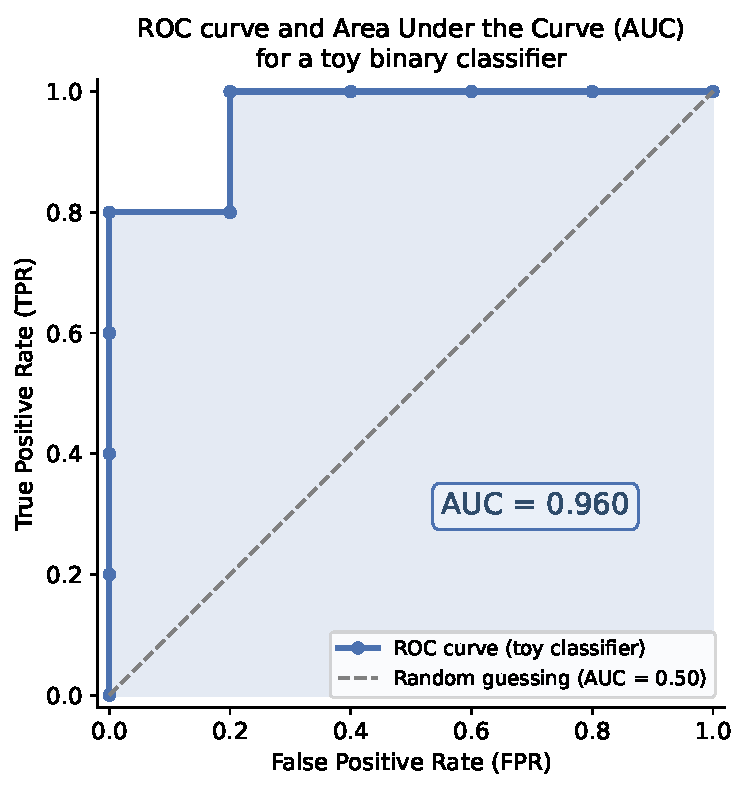
\includegraphics[width=0.62\linewidth]{fig_roc_auc.pdf}

  \small The staircase ROC curve for the toy classifier above, the
  $45^\circ$ diagonal representing random guessing (AUC $=0.5$), and the
  computed AUC $\approx 0.960$ marked on the plot.
\end{frame}

% -----------------------------------------------------------------------------
\begin{frame}[allowframebreaks]{Regression Metrics: $R^2$, MAE, MSE (and RMSE)}
  \begin{block}{Mean Squared Error (MSE) and Root MSE}
    \[
      \text{MSE} = \frac{1}{n}\sum_{i=1}^{n}(y_i - \hat y_i)^2, \qquad
      \text{RMSE} = \sqrt{\text{MSE}}
    \]
    $y_i$: observed (true) value; $\hat y_i$: model's forecast; $n$: number
    of observations. MSE (and its square root, RMSE, in the same units as
    $y$) quantify the average squared difference between observations and
    forecasts -- \emph{low} values indicate a good model.
  \end{block}

  \begin{block}{Mean Absolute Error (MAE)}
    \[
      \text{MAE} = \frac{1}{n}\sum_{i=1}^{n}\left|y_i-\hat y_i\right|
    \]
    Similar to MSE/RMSE, but penalizes large errors less severely (no
    squaring). Low MAE indicates a good model.
  \end{block}

  \framebreak

  \begin{block}{Coefficient of Determination ($R^2$)}
    \[
      R^2 = 1 - \frac{\sum_{i=1}^n (y_i-\hat y_i)^2}{\sum_{i=1}^n (y_i-\bar y)^2},
      \qquad \bar y = \frac{1}{n}\sum_{i=1}^n y_i
    \]
    $R^2$ indicates the percentage of the target variable's variability that
    the model explains. High $R^2$ (close to $1$) indicates a good model.
  \end{block}

  \textbf{Toy example.} $y = [3,5,2,7,4]$, $\hat y = [2.5,5.5,2,6,4.5]$.
  Residuals: $e=[0.5,-0.5,0,1,-0.5]$.
  \[
    \text{MSE} = \frac{0.25+0.25+0+1+0.25}{5} = 0.35, \qquad
    \text{RMSE} = \sqrt{0.35} \approx 0.592,
  \]
  \[
    \text{MAE} = \frac{0.5+0.5+0+1+0.5}{5} = 0.5, \qquad \bar y = 4.2,
  \]
  \[
    R^2 = 1 - \frac{1.75}{14.8} \approx 0.882.
  \]
  Small errors (MSE, RMSE, MAE all modest) and a high $R^2$ ($0.882$, i.e.\
  the model explains $88.2\%$ of the variability in $y$) together indicate
  a good regression fit.
\end{frame}

% -----------------------------------------------------------------------------
\begin{frame}[fragile]{Python: Computing All Performance Metrics by Hand}
  \begin{lstlisting}
import numpy as np

# --- classification toy set ---
y_true  = np.array([1,1,1,1,0,1,0,0,0,0])
y_score = np.array([.92,.85,.78,.66,.61,.55,.48,.42,.30,.11])
y_pred  = (y_score >= 0.5).astype(int)

TP = np.sum((y_pred==1) & (y_true==1)); FP = np.sum((y_pred==1) & (y_true==0))
TN = np.sum((y_pred==0) & (y_true==0)); FN = np.sum((y_pred==0) & (y_true==1))

accuracy  = (TP+TN)/len(y_true)
precision = TP/(TP+FP)
recall    = TP/(TP+FN)
f_measure = 2*precision*recall/(precision+recall)
print(f"Acc={accuracy:.3f} Prec={precision:.3f} Rec={recall:.3f} F1={f_measure:.3f}")

# --- regression toy set ---
y, y_hat = np.array([3,5,2,7,4]), np.array([2.5,5.5,2,6,4.5])
resid = y - y_hat
mse, mae = np.mean(resid**2), np.mean(np.abs(resid))
r2 = 1 - np.sum(resid**2)/np.sum((y-y.mean())**2)
print(f"MSE={mse:.4f} RMSE={np.sqrt(mse):.4f} MAE={mae:.4f} R2={r2:.4f}")
  \end{lstlisting}
  \textbf{Output:} {\ttfamily Acc=0.900 Prec=0.833 Rec=1.000 F1=0.909} and
  {\ttfamily MSE=0.3500 RMSE=0.5916 MAE=0.5000 R2=0.8818} -- matching every
  hand computation on the previous slides exactly.
\end{frame}

% =============================================================================
\section{2.3 Conclusion}
% =============================================================================

\begin{frame}[allowframebreaks]{2.3 Conclusion}
  This chapter introduced:
  \begin{itemize}
    \item the \textbf{Bayesian framework} and how it differs from the
      frequentist paradigm (Table 2.1);
    \item typical \textbf{Bayesian machine learning models} -- Bayesian
      logistic regression, Bayesian mixture models, Gaussian processes,
      Bayesian neural networks, and Bayesian formulations of economic
      models -- plus two further tools (normalizing flows, and deeper BNN
      machinery) previewed for later chapters;
    \item how to \textbf{train} these models, focusing on the two main
      approaches: \textbf{variational inference} (an optimization
      problem, via the ELBO) and \textbf{Markov Chain Monte Carlo}
      (a sampling problem, via a guided random walk); and
    \item the \textbf{performance metrics} used throughout the book:
      multivariate ESS and ESS/time for MCMC sampling efficiency; accuracy,
      precision, recall, F-measure, ROC and AUC for classification; and
      $R^2$, MAE, MSE for regression.
  \end{itemize}

  \framebreak

  \textbf{Looking ahead.} In the next chapter, we calibrate the Stochastic
  Alpha Beta Rho (SABR) stochastic volatility model using Bayesian methods,
  and show the benefits of this in terms of uncertainty quantification --
  without loss of model accuracy. Every term introduced in this chapter
  (posterior, likelihood, prior, evidence, MCMC, variational inference,
  Gaussian processes, normalizing flows, Bayesian neural networks, and the
  performance metrics above) will be used without further re-explanation
  from here on.
\end{frame}

% -----------------------------------------------------------------------------
\begin{frame}[allowframebreaks]{Recap: Key Vocabulary Checklist}
  \small
  \begin{itemize}
    \item \textbf{Bayesian machine learning}: fitting a model \emph{and}
      obtaining a full distribution over its uncertainty, not just one
      best-fit answer.
    \item \textbf{Prior / likelihood / posterior}: belief before data /
      probability of data given parameters / belief after data.
    \item \textbf{Bayesian evidence}: the normalizing constant
      $\mathbb{P}(D\mid M)$; useful for model selection.
    \item \textbf{Variational inference}: approximate the posterior with a
      simpler distribution $Q$, and find the best member of that family by
      maximizing the ELBO (an optimization problem).
    \item \textbf{MCMC}: draw samples from the posterior by running a
      cleverly designed random walk whose stationary distribution is the
      posterior (a sampling problem); Metropolis-Hastings is the seminal
      algorithm, HMC/NUTS/MHMC/S2HMC are its modern descendants.
    \item \textbf{Gaussian process}: a non-parametric ``distribution over
      functions.''
    \item \textbf{Normalizing flow}: build a complex distribution by pushing
      a simple one (e.g.\ Gaussian) through invertible transformations.
    \item \textbf{Bayesian neural network}: a neural network with a
      distribution over its weights, not fixed numbers.
    \item \textbf{Performance metrics}: (multivariate) ESS and ESS/time for
      MCMC efficiency; accuracy / precision / recall / F-measure / ROC /
      AUC for classification; $R^2$ / MAE / MSE for regression.
  \end{itemize}
\end{frame}

% -----------------------------------------------------------------------------
\begin{frame}{References}
  \small
  \begin{thebibliography}{9}
    \bibitem{mongwe2025}
      W. T. Mongwe, R. Mbuvha, and T. Marwala,
      \textit{Bayesian Machine Learning in Quantitative Finance: Theory and
      Practical Applications}. Springer, 2025.
    \bibitem{hastings1970}
      W. K. Hastings,
      ``Monte Carlo Sampling Methods Using Markov Chains and Their
      Applications,'' \textit{Biometrika}, 57(1), 97--109, 1970.
    \bibitem{hoffman2014}
      M. D. Hoffman and A. Gelman,
      ``The No-U-Turn Sampler: Adaptively Setting Path Lengths in
      Hamiltonian Monte Carlo,'' \textit{JMLR}, 15(1), 1593--1623, 2014.
    \bibitem{blei2017}
      D. M. Blei, A. Kucukelbir, and J. D. McAuliffe,
      ``Variational Inference: A Review for Statisticians,''
      \textit{JASA}, 112(518), 859--877, 2017.
    \bibitem{marwala2023}
      T. Marwala, R. Mbuvha, and W. T. Mongwe,
      \textit{Hamiltonian Monte Carlo Methods in Machine Learning}.
      Elsevier, 2023.
    \bibitem{vats2019}
      D. Vats, J. M. Flegal, and G. L. Jones,
      ``Multivariate Output Analysis for Markov Chain Monte Carlo,''
      \textit{Biometrika}, 106(2), 321--337, 2019.
    \bibitem{bharadiya2023}
      J. P. Bharadiya,
      ``A Review of Bayesian Machine Learning Principles, Methods, and
      Applications,'' \textit{International Journal of Innovative Science
      and Research Technology}, 8(5), 2033--2038, 2023.
    \bibitem{mackay1992}
      D. J. C. MacKay,
      ``A Practical Bayesian Framework for Backpropagation Networks,''
      \textit{Neural Computation}, 4(3), 448--472, 1992.
  \end{thebibliography}
\end{frame}

\end{document}
